\chapter{Projektmanagement}
\section{Entscheidung}
Die Entscheidung der Projektmanagementmethode ist sehr wichtig und sollte sorgfältig gemacht werden. Sollte eine Methode falsch angewandt werden, kann sie das Team verlangsamen und bei der Arbeit hindern. Bei dieser Entscheidung hilft die Stacey Matrix.

\begin{wrapfigure}[15]{r}[0pt]{0.5\textwidth}
  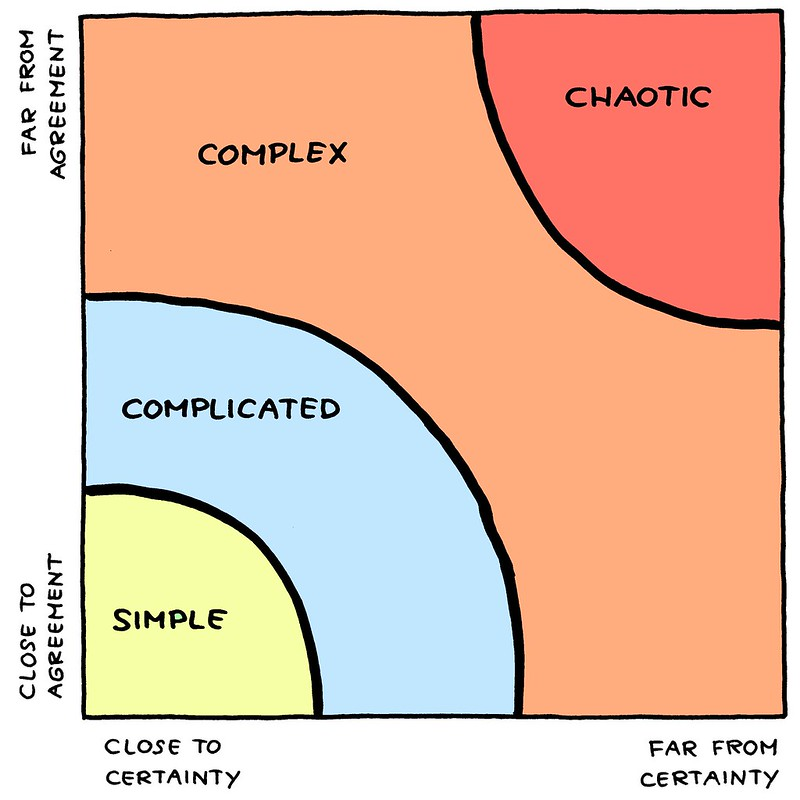
\includegraphics[width=0.9\linewidth]{./images/stacey_matrix}
  \caption[\href{https://blog.ordix.de/welches-vorgehen-eignet-sich-fuer-mein-projekt}{Stacey Matrix Grafik von Jurgen Appello.}]{Stacey Matrix}
  \label{fig:stacey}
\end{wrapfigure}\leavevmode

Die x-Achse beschreibt, wie klar der Auftrag ist. Das heisst, ob alle Anforderungen gegeben sind oder noch welche zu einem späteren Zeitpunkt dazu kommen. Die y-Achse beschreibt dagegen, wie deutlich der Weg zu diesen Kriterien ist. Dabei fragt sich zum Beispiel, ob es klar ist, wie man den Auftrag mit dieser Programmiersprache/diesem Framework lösen kann.
\newline
Die ganze Auswertung beruht auf Schätzungen. Diese subjektiven Beobachtungen werden allerdings präziser, je mehr Berufserfahrung man sammelt.
\newline
In der Abbildung \ref*{fig:stacey} gibt es vier Abschnitte. Je nachdem, wo man landet, sollte man eine andere Projektmanagementmethode anwenden.
\newpage
\begin{itemize}
  \item \textbf{Simpel} - Das Ziel und der Weg dahin sind klar. In diesem Fall sollte das Wasserfallmodell oder eine ähnliche Methode gewählt werden.
  \item \textbf{Kompliziert} - Sollte entweder das Ziel oder der Lösungsweg etwas unklar sein, sollte man Kanban anwenden.
  \item \textbf{Komplex} - Sind beide Achsen unklar oder ändern sich Kriterien, sollte etwas Agiles wie Scrum gewählt werden. Eine Methode wie diese ist für wechselnde Anforderungen gemacht.
  \item \textbf{Chaotisch} - Das Ziel und der Weg dahin sind unklar. In diesem Fall sollte das Projekt noch nicht gestartet werden. Stattdessen sollte für mehr Klarheit an beiden Achsen gesorgt werden. 
\end{itemize}

\section{Wasserfallmodell}

\begin{figure}[!ht]
  \centering
  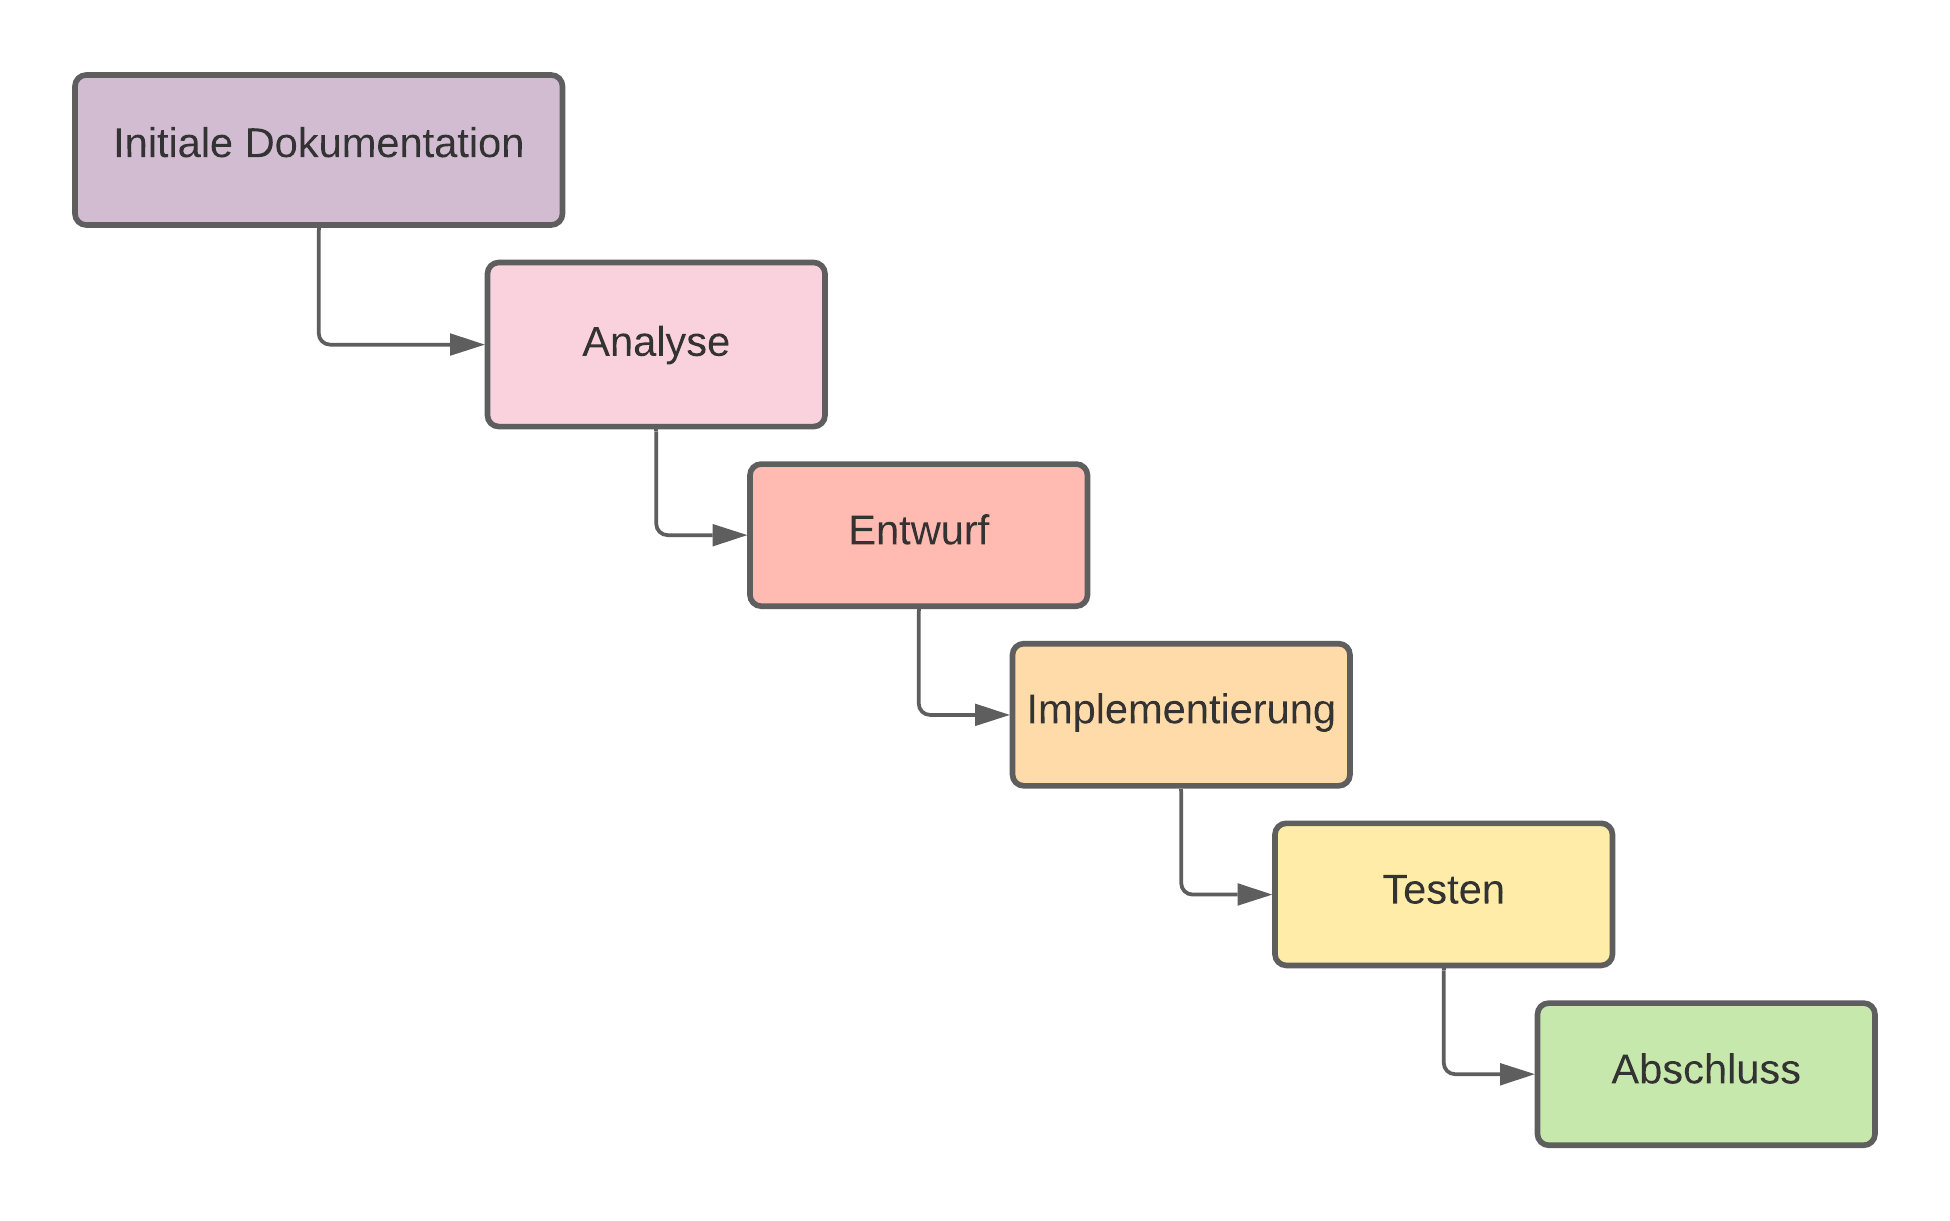
\includegraphics[width=.95\linewidth]{./images/OSEDashboard_Wasserfall.png}
  \caption[Ein von mir mit Lucidchart erstelltes Wasserfallmodell]{Wasserfall Modell}
  \label{fig:wasserfall}
\end{figure}

Das Wasserfallmodell arbeitet mit auf sich selber aufbauenden sequenziellen Phasen. Man beginnt erst
mit dem nächsten Stadium, sobald die Letzte komplett abgeschlossen ist. Dies erfordert, dass das Ziel und
der Weg dorthin klar sein muss. Ein streng geregelter Arbeitsablauf mit Meilensteinen kann dadurch
ermöglicht werden, was vorallem für kleine Projekte wie dieses sehr nützlich ist.

\subsection{Initialisierung des Dokuments}

Als Erstes soll das Dokument für die kommenden Arbeitstage so vorbereitet werden, dass mir nachher nichts mehr im Weg steht. Zuerst habe ich die LaTeX-Vorlage nochmals angesehen, um sicherzugehen, dass alles stimmt und richtig konfiguriert ist. Danach sollten essenzielle Bestandteile wie der detaillierte Zeitplan, das Arbeitsjournal und der obligatorische Teil erstellt werden. Dies habe ich soweit verfasst. Nun fehlt nur noch dieses Kapitel und dieser Arbeitsschritt ist abgeschlossen.

\subsection{Analyse}

Nachdem die Initialisierung komplett abgeschlossen ist, geht es dann an die Analyse. Diese beinhaltet unter anderem eine Systembeschreibung, ein Ist/Soll-Vergleich, Konzepte wie ich die Sicherung der Arbeitsergebnisse sicherstelle und die OAuth2-Strategie. Ersteres beschreibt, wie genau unser Netilion-Ökosystem funktioniert und wie dieses Projekt darin integriert werden soll. Der Ist/Soll-Vergleich zeigt nochmals die zu erarbeitende Lösung auf und wie sie sich mit dem bereits existierenden Produkt differenziert. Die OAuth2-Strategie soll genau beschreiben, wie der Anmeldeprozess abläuft und was ihn sicher macht.
\newline
Ausserdem enthalten sind Personas und detaillierte User-Stories. Diese werden gebildet, indem die Anforderung des Auftraggebers in kleinere Stücke aufgebrochen werden, damit sich der Entwickler auf einzelne Entwicklungsabschnitte konzentrieren kann und der Fortschritt messbarer wird.

\subsubsection{User-Stories}

Die User Story beschreibt in kurzer Form eine Anforderung einer Anspruchsgruppe an die Software. Dabei soll geklärt werden, \textbf{wer} welche \textbf{Funktionalität} aus welchem \textbf{Grund} implementiert haben möchte. Ohne dabei zu sehr in technische Details zu gehen, beschreibt sie, was genau von der Software gefordert ist. Dies ermöglicht eine einfachere Absprache mit den Anspruchsgruppen. Wie dabei diese Anforderungen implementiert werden, spielt keine Rolle. Sehr oft wird diese kurze Beschreibung als Titel für eine Story im Projektmanagementtool genommen.

\textbf{Beispiel einer User Story:}
\newline
Als \textit{<Anspruchsgruppe>} möchte ich \textit{<Feature>}, damit \textit{<Anwendungsfall>} erreicht wird.
\linebreak
\linebreak
Als \textit{Nutzer} möchte ich, dass \textit{die ne107 Werte grafisch dargestellt werden} , damit \textit{ich die Status der Messgeräte direkt sehen kann}.

\subsection{Entwurf}

In der Entwurfsphase wird der genaue Lösungsweg ermittelt. Der Entwickler beschreibt, wie er mit welchen technischen Mitteln die zuvor definierten Ziele erreichen kann. Teil davon ist auch, welche Mittel er einsetzt, wieso er diese verwendet und wie er sie anwenden will. Dazu gehören Schnittstellen, Bibliotheken, Datenbank und so weiter. Das Ergebnis dieser Phase ist ein ausgearbeitetes UI/UX Design, genaue Pläne, wie die Software aufgebaut werden soll und das Testkonzept.

\subsection{Implementierung}

In diesem Abschnitt gilt es, die dokumentierten Anforderungen mit den gewählten Technologien umzusetzen. Dabei sollen die User-Stories und Testfälle von den vorherigen Kapiteln beachtet werden.
\newline
Nachdem eine Story abgeschlossen ist, wird die Änderung auf einen Branch gepusht und automatisch deployed. So können die Anspruchsgruppen zeitnahe Rückmeldungen geben. Das Produkt der Implementierungsphase ist die fertige Software.


\subsection{Testen}

In dieser Phase wird nochmals sorgfältig durchgegangen, ob alle Kriterien erfüllt wurden und ob die Tests wie gewünscht ablaufen. Stimmt das Ergebnis mit den gesetzten Erwartungen, gilt die Software als fertiggestellt.

\subsection{Abschluss}

Nachdem alle Ziele erreicht und mit dem Testprotokoll verifiziert wurden, soll die restliche Zeit für die Überarbeitung/Verbesserung der Dokumentation eingesetzt werden. Anschliesend soll die IPA am 14.04.2021 abgegeben werden.